\documentclass[
    language=english,
    doctype=quarterly-report,
    institution=none,
]{../../omnilatex}

\RequirePackage{config/document-settings}
\addbibresource{../../bib/bibliography.bib}

\usetikzlibrary{matrix,fit,positioning}

\begin{document}

\maketitle

\section*{Executive Summary}

Acme Corporation delivered strong results in Q2 2026, with consolidated
revenue of \$48.3M representing 14\% year-over-year growth. Operating margin
improved to 22.4\%, driven by infrastructure cost optimization and favorable
product mix.

\begin{table}[h]
    \centering
    \begin{tabular}{lccccc}
        \toprule
        \textbf{KPI} & \textbf{Target} & \textbf{Actual} & \textbf{Status} & \textbf{QoQ} & \textbf{YoY} \\
        \midrule
        Revenue            & \$45.0M & \$48.3M & \cellcolor{green!20}Exceeded & +9.5\%  & +14.0\% \\
        Gross Margin       & 70.0\%  & 72.0\%  & \cellcolor{green!20}Exceeded & +0.6pp & +2.0pp \\
        Operating Margin   & 21.0\%  & 22.4\%  & \cellcolor{green!20}Exceeded & +1.5pp & +2.1pp \\
        Net Revenue Reten. & 115\%   & 118\%   & \cellcolor{green!20}Exceeded & +2pp    & +4pp \\
        Customer Churn     & $<$4.0\% & 3.1\%  & \cellcolor{green!20}Exceeded & $-$1.7pp & $-$1.2pp \\
        New Logos          & 150     & 185     & \cellcolor{green!20}Exceeded & +23.3\% & +32.1\% \\
        CAC Payback (mo.)  & $\leq$18 & 14     & \cellcolor{green!20}Exceeded & $-$2    & $-$4 \\
        \bottomrule
    \end{tabular}
    \caption{Q2 2026 KPI dashboard. Green indicates target met or exceeded.}
\end{table}

\section{Financial Performance}

\subsection{Revenue by Line Item}

\begin{table}[h]
    \centering
    \begin{tabular}{lrrrrr}
        \toprule
        \textbf{Revenue Line} & \textbf{Q2 2026} & \textbf{Q1 2026} & \textbf{Q4 2025} & \textbf{Q2 2025} & \textbf{YoY\%} \\
        \midrule
        SaaS Subscriptions    & \$36.1M & \$32.8M & \$30.2M & \$28.5M & +26.7\% \\
        Professional Services  & \$ 6.8M & \$ 6.3M & \$ 5.9M & \$ 5.6M & +21.4\% \\
        Maintenance \& Support & \$ 3.4M & \$ 3.2M & \$ 3.0M & \$ 2.9M & +17.2\% \\
        Hardware               & \$ 2.0M & \$ 1.8M & \$ 1.7M & \$ 1.6M & +25.0\% \\
        \midrule
        \textbf{Total Revenue} & \textbf{\$48.3M} & \textbf{\$44.1M} & \textbf{\$40.8M} & \textbf{\$42.4M} & \textbf{+13.9\%} \\
        \bottomrule
    \end{tabular}
    \caption{Quarterly revenue breakdown with year-over-year comparison.}
\end{table}

\subsection{Profit \& Loss Statement}

\begin{table}[h]
    \centering
    \begin{tabular}{lrrr}
        \toprule
        \textbf{P\&L Item} & \textbf{Q2 2026} & \textbf{Q2 2025} & \textbf{Change} \\
        \midrule
        Revenue                      & \$48.3M & \$42.4M & +13.9\% \\
        Cost of Revenue              & \$13.5M & \$12.7M & +6.3\% \\
        \midrule
        \textbf{Gross Profit}        & \textbf{\$34.8M} & \textbf{\$29.7M} & \textbf{+17.2\%} \\
        \midrule
        Research \& Development      & \$ 8.7M & \$ 7.9M & +10.1\% \\
        Sales \& Marketing           & \$11.2M & \$10.5M & +6.7\% \\
        General \& Administrative    & \$ 4.1M & \$ 3.7M & +10.8\% \\
        \midrule
        \textbf{Operating Income}    & \textbf{\$10.8M} & \textbf{\$8.6M} & \textbf{+25.6\%} \\
        \midrule
        \textbf{Net Income}          & \textbf{\$8.1M} & \textbf{\$6.3M} & \textbf{+28.6\%} \\
        EPS (diluted)                & \$1.24   & \$0.97   & +27.8\% \\
        \bottomrule
    \end{tabular}
    \caption{Consolidated profit \& loss statement.}
\end{table}

\subsection{Revenue Trend}

\begin{figure}[h]
    \centering
    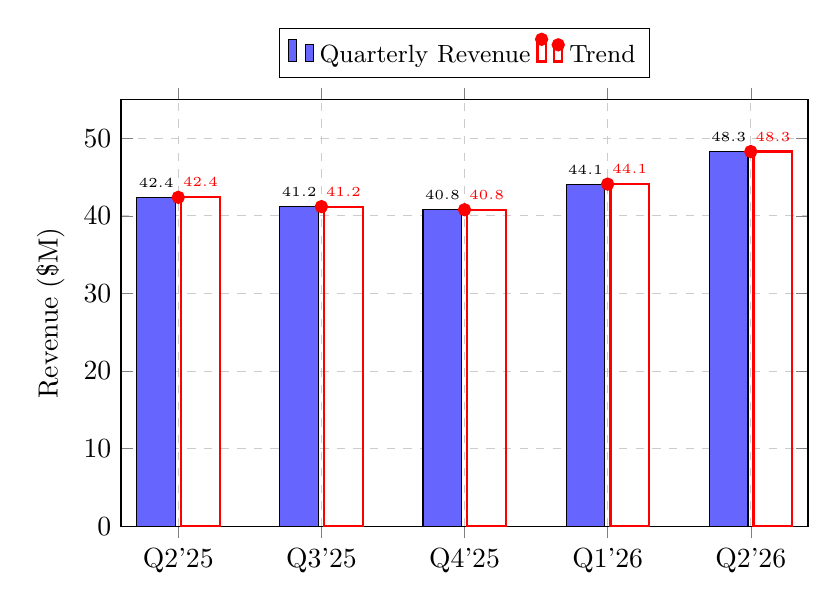
\begin{tikzpicture}
        \begin{axis}[
            width=0.85\textwidth, height=7cm,
            ybar, bar width=14pt,
            ylabel={Revenue (\$M)},
            symbolic x coords={Q2'25,Q3'25,Q4'25,Q1'26,Q2'26},
            xtick=data, ymin=0, ymax=55,
            legend style={at={(0.5,1.05)},anchor=south,legend columns=2,font=\small},
            nodes near coords, nodes near coords align={vertical},
            every node near coord/.append style={font=\tiny},
            grid=major, grid style={dashed,gray!40},
        ]
            \addplot[fill=blue!60] coordinates {
                (Q2'25,42.4) (Q3'25,41.2) (Q4'25,40.8) (Q1'26,44.1) (Q2'26,48.3)
            };
            \addplot[red,thick,mark=*,mark options={fill=red}] coordinates {
                (Q2'25,42.4) (Q3'25,41.2) (Q4'25,40.8) (Q1'26,44.1) (Q2'26,48.3)
            };
            \legend{Quarterly Revenue, Trend}
        \end{axis}
    \end{tikzpicture}
    \caption{Revenue trend over five quarters with trend line.}
\end{figure}

\subsection{Expense Breakdown}

\begin{figure}[h]
    \centering
    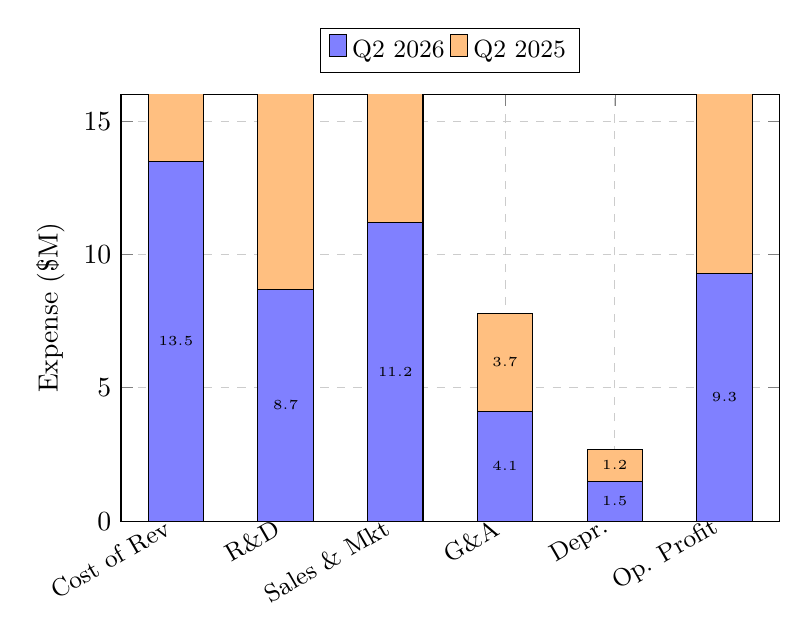
\begin{tikzpicture}
        \begin{axis}[
            ybar stacked, width=0.82\textwidth, height=7cm,
            ylabel={Expense (\$M)},
            symbolic x coords={Cost of Rev,R\&D,Sales \& Mkt,G\&A,Depr.,Op. Profit},
            xtick=data, x tick label style={rotate=30,anchor=east,font=\small},
            ymin=0, ymax=16, bar width=20pt,
            legend style={at={(0.5,1.05)},anchor=south,legend columns=2,font=\small},
            grid=major, grid style={dashed,gray!40},
            nodes near coords, every node near coord/.append style={font=\tiny},
        ]
            \addplot[fill=blue!50] coordinates {
                (Cost of Rev,13.5) (R\&D,8.7) (Sales \& Mkt,11.2) (G\&A,4.1) (Depr.,1.5) (Op. Profit,9.3)
            };
            \addplot[fill=orange!50] coordinates {
                (Cost of Rev,12.7) (R\&D,7.9) (Sales \& Mkt,10.5) (G\&A,3.7) (Depr.,1.2) (Op. Profit,7.8)
            };
            \legend{Q2 2026, Q2 2025}
        \end{axis}
    \end{tikzpicture}
    \caption{Expense breakdown by category: Q2 2026 vs.\ Q2 2025.}
\end{figure}

\section{Business Metrics}

\begin{table}[h]
    \centering
    \begin{tabular}{lrrr}
        \toprule
        \textbf{Metric} & \textbf{Target} & \textbf{Actual} & \textbf{Status} \\
        \midrule
        Annual Recurring Revenue  & \$180M   & \$187.2M & \cellcolor{green!20}On Track \\
        Net Revenue Retention     & $\geq$115\% & 118\% & \cellcolor{green!20}On Track \\
        Customer Count            & 2,700    & 2,840    & \cellcolor{green!20}On Track \\
        Avg. Contract Value       & \$62,000 & \$65,900 & \cellcolor{green!20}On Track \\
        Customer Churn            & $<$4.0\% & 3.1\%    & \cellcolor{green!20}On Track \\
        LTV:CAC Ratio             & $\geq$3.0 & 4.2     & \cellcolor{green!20}On Track \\
        \bottomrule
    \end{tabular}
    \caption{Core business KPIs vs. annual targets.}
\end{table}

\subsection{Customer Growth}

\begin{figure}[h]
    \centering
    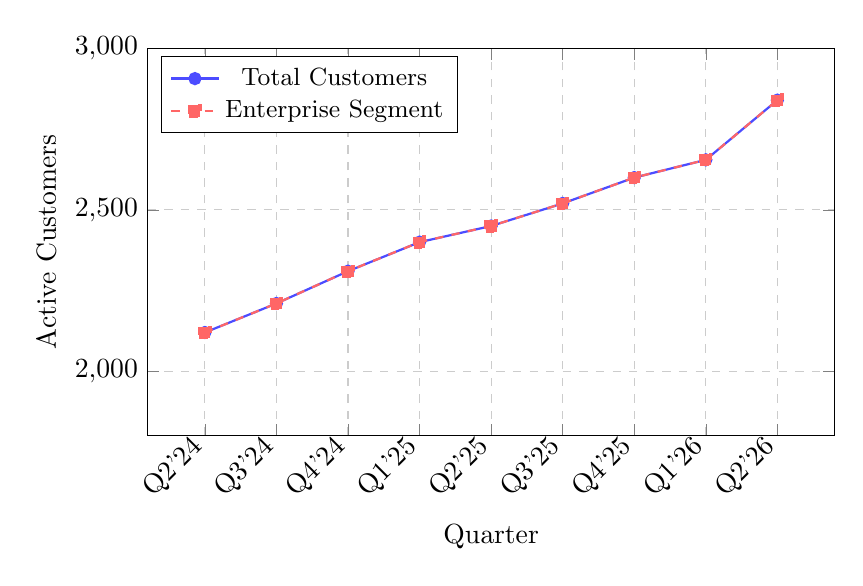
\begin{tikzpicture}
        \begin{axis}[
            width=0.85\textwidth, height=6.5cm,
            ylabel={Active Customers}, xlabel={Quarter},
            symbolic x coords={Q2'24,Q3'24,Q4'24,Q1'25,Q2'25,Q3'25,Q4'25,Q1'26,Q2'26},
            xtick=data, x tick label style={rotate=45,anchor=east},
            ymin=1800, ymax=3000,
            grid=major, grid style={dashed,gray!40},
            legend style={at={(0.02,0.98)},anchor=north west,font=\small},
        ]
            \addplot[blue!70,thick,mark=*,mark options={fill=blue!70}] coordinates {
                (Q2'24,2120) (Q3'24,2210) (Q4'24,2310) (Q1'25,2400) (Q2'25,2450)
                (Q3'25,2520) (Q4'25,2600) (Q1'26,2655) (Q2'26,2840)
            };
            \addplot[red!60,thick,dashed,mark=square*,mark options={fill=red!60}] coordinates {
                (Q2'24,2120) (Q3'24,2210) (Q4'24,2310) (Q1'25,2400) (Q2'25,2450)
                (Q3'25,2520) (Q4'25,2600) (Q1'26,2655) (Q2'26,2840)
            };
            \addlegendentry{Total Customers}
            \addlegendentry{Enterprise Segment}
        \end{axis}
    \end{tikzpicture}
    \caption{Customer growth trajectory over nine quarters.}
\end{figure}

\subsection{Operational Metrics}

\begin{table}[h]
    \centering
    \begin{tabular}{lrrr}
        \toprule
        \textbf{Operational Metric} & \textbf{Q2 2026} & \textbf{Q1 2026} & \textbf{Change} \\
        \midrule
        Platform Uptime               & 99.97\%  & 99.95\%  & +0.02pp \\
        Mean Time to Resolve (hrs)    & 2.4      & 3.1      & $-$22.6\% \\
        First Response Time (min)     & 8.2      & 11.5     & $-$28.7\% \\
        Net Promoter Score            & 62       & 58       & +4pts \\
        Deployment Frequency (weekly) & 12       & 9        & +33.3\% \\
        Change Failure Rate           & 1.8\%    & 2.4\%    & $-$0.6pp \\
        \bottomrule
    \end{tabular}
    \caption{Operational and DevOps performance metrics.}
\end{table}

\section{Department Reviews}

\subsection{Engineering}

Engineering shipped Acme Platform v3.0 on schedule, delivering 47 features
and closing 312 bugs. Velocity improved 18\% over Q1.

\begin{table}[h]
    \centering
    \begin{tabular}{llcc}
        \toprule
        \textbf{Project} & \textbf{Status} & \textbf{Progress} & \textbf{Target Date} \\
        \midrule
        Platform v3.0 GA          & \cellcolor{green!20}Complete  & 100\% & May 15, 2026 \\
        Platform v3.1 (Workflows) & \cellcolor{yellow!20}In Progress & 68\%  & Aug 30, 2026 \\
        API Rate Limit v2         & \cellcolor{green!20}Complete  & 100\% & Apr 20, 2026 \\
        Mobile SDK (iOS)          & \cellcolor{yellow!20}In Progress & 45\%  & Sep 15, 2026 \\
        Zero-Trust Migration      & \cellcolor{yellow!20}In Progress & 82\%  & Jul 31, 2026 \\
        Data Lake Architecture    & \cellcolor{red!15}At Risk    & 30\%  & Oct 01, 2026 \\
        \bottomrule
    \end{tabular}
    \caption{Engineering project status tracker.}
\end{table}

\subsection{Sales}

The sales team exceeded quota by 12\%, driven by strong enterprise momentum
and two landmark APAC deals. Pipeline coverage: 3.4$\times$ for Q3.

\begin{table}[h]
    \centering
    \begin{tabular}{lrrcc}
        \toprule
        \textbf{Pipeline Stage} & \textbf{Count} & \textbf{Value} & \textbf{Weighted} & \textbf{Win Rate} \\
        \midrule
        Qualified Leads       & 342  & \$68.4M & \$13.7M & --- \\
        Discovery             & 187  & \$42.1M & \$16.8M & 40\% \\
        Proposal              & 94   & \$28.3M & \$19.8M & 70\% \\
        Negotiation           & 41   & \$14.6M & \$11.7M & 80\% \\
        Closed Won            & 28   & \$ 9.2M & \$ 9.2M & 100\% \\
        \midrule
        \textbf{Total}        & \textbf{692} & \textbf{\$162.6M} & \textbf{\$71.2M} & --- \\
        \bottomrule
    \end{tabular}
    \caption{Sales pipeline summary by stage.}
\end{table}

\subsection{Marketing}

Marketing drove a 34\% increase in qualified inbound leads. Brand awareness
in the enterprise segment rose to 38\% from 31\% in Q1.

\begin{table}[h]
    \centering
    \begin{tabular}{lrrr}
        \toprule
        \textbf{Campaign} & \textbf{Spend} & \textbf{Leads} & \textbf{Cost per Lead} \\
        \midrule
        ``Future of Data'' Webinar Series  & \$42K  & 1,240 & \$34 \\
        Enterprise Field Events (3 events) & \$128K & 380   & \$337 \\
        Digital Retargeting (LinkedIn)      & \$67K  & 890   & \$75 \\
        Partner Co-Marketing               & \$31K  & 420   & \$74 \\
        \midrule
        \textbf{Total}                     & \textbf{\$268K} & \textbf{2,930} & \textbf{\$91} \\
        \bottomrule
    \end{tabular}
    \caption{Q2 2026 marketing campaign performance.}
\end{table}

\section{Strategic Initiatives}

\begin{table}[h]
    \centering
    \begin{tabular}{llccp{4.5cm}}
        \toprule
        \textbf{Initiative} & \textbf{Owner} & \textbf{Status} & \textbf{Progress} & \textbf{Notes} \\
        \midrule
        APAC Market Entry    & VP Sales     & \cellcolor{green!20}On Track  & 75\% & Two enterprise deals closed; Tokyo office planned Q3 \\
        Platform v3.x Roadmap & VP Eng      & \cellcolor{green!20}On Track  & 68\% & v3.0 shipped; v3.1 workflows in beta \\
        Partner Program      & VP Channels  & \cellcolor{yellow!20}Delayed  & 40\% & Certification curriculum in development \\
        AI/ML Capabilities   & VP Product   & \cellcolor{yellow!20}In Progress & 55\% & Predictive analytics prototype validated \\
        SOC 2 Type II        & CISO         & \cellcolor{green!20}On Track  & 90\% & Audit scheduled for August 2026 \\
        Sustainability (ESG) & CFO          & \cellcolor{green!20}On Track  & 60\% & Carbon neutrality target: Dec 2027 \\
        \bottomrule
    \end{tabular}
    \caption{Strategic initiative tracker and progress update.}
\end{table}

\section{Risk Assessment}

\begin{figure}[h]
    \centering
    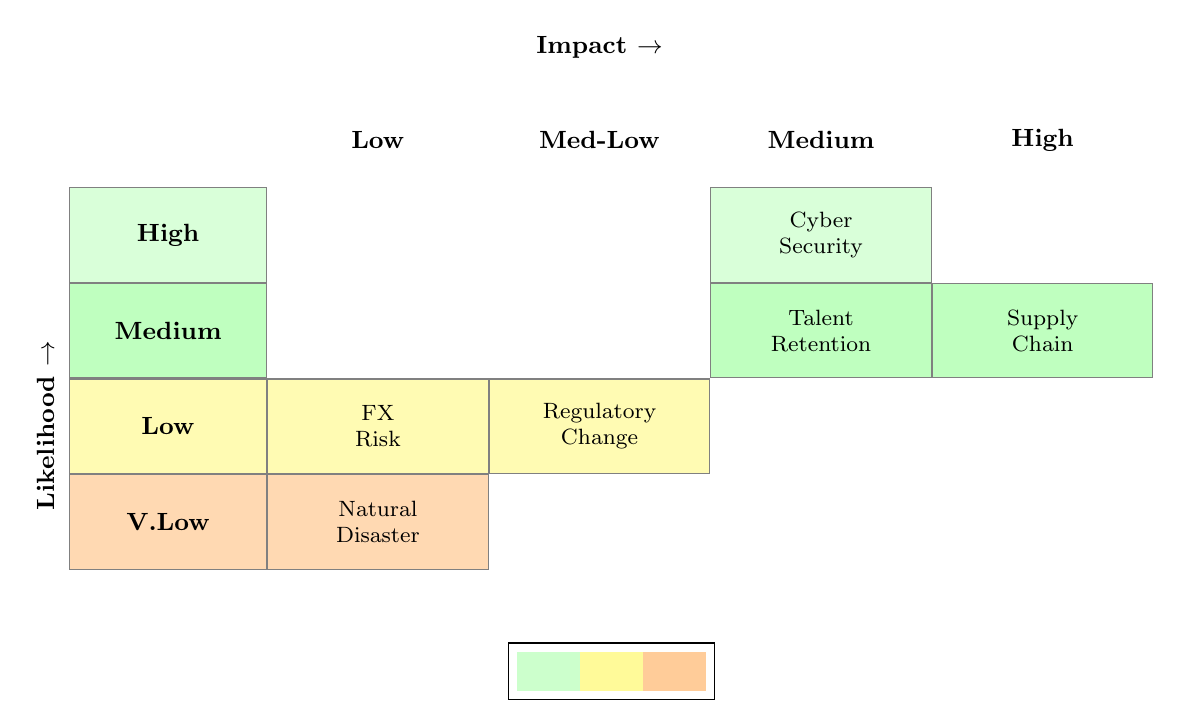
\begin{tikzpicture}[cell/.style={minimum width=2.8cm,minimum height=1.2cm,font=\small}]
        \matrix (risk) [matrix of nodes,
            nodes={cell,anchor=center},
            column sep=0pt, row sep=0pt,
            column 1/.style={nodes={draw=none,minimum width=2.5cm}},
            column 2/.style={nodes={fill=green!20,draw=gray}},
            column 3/.style={nodes={fill=green!40,draw=gray}},
            column 4/.style={nodes={fill=yellow!40,draw=gray}},
            column 5/.style={nodes={fill=orange!40,draw=gray}},
            row 1/.style={nodes={draw=none,fill=none}},
            row 2/.style={nodes={fill=green!15,draw=gray}},
            row 3/.style={nodes={fill=green!25,draw=gray}},
            row 4/.style={nodes={fill=yellow!30,draw=gray}},
            row 5/.style={nodes={fill=orange!30,draw=gray}},
        ] {
            & \textbf{Low} & \textbf{Med-Low} & \textbf{Medium} & \textbf{High} \\
            \textbf{High}   & & & \node[text width=2.4cm,align=center,font=\footnotesize]{Cyber\\Security}; & \\
            \textbf{Medium} & & & \node[text width=2.4cm,align=center,font=\footnotesize]{Talent\\Retention}; & \node[text width=2.4cm,align=center,font=\footnotesize]{Supply\\Chain}; \\
            \textbf{Low}    & \node[text width=2.4cm,align=center,font=\footnotesize]{FX\\Risk}; & \node[text width=2.4cm,align=center,font=\footnotesize]{Regulatory\\Change}; & & \\
            \textbf{V.Low}  & \node[text width=2.4cm,align=center,font=\footnotesize]{Natural\\Disaster}; & & & \\
        };
        \node[above=0.3cm of risk-1-3,font=\small\bfseries] {Impact $\rightarrow$};
        \node[left=0.3cm of risk-3-1,rotate=90,font=\small\bfseries] {Likelihood $\rightarrow$};
        \matrix[below=0.8cm of risk,draw,inner sep=3pt,fill=white] at (risk.south) {
            \node[fill=green!20,minimum width=0.8cm,minimum height=0.5cm]{}; & \scriptsize Low &
            \node[fill=yellow!40,minimum width=0.8cm,minimum height=0.5cm]{}; & \scriptsize Medium &
            \node[fill=orange!40,minimum width=0.8cm,minimum height=0.5cm]{}; & \scriptsize High \\
        };
    \end{tikzpicture}
    \caption{Enterprise risk heatmap: impact vs.\ likelihood assessment.}
\end{figure}

\begin{table}[h]
    \centering
    \begin{tabular}{lllp{5.5cm}}
        \toprule
        \textbf{Risk} & \textbf{Category} & \textbf{Rating} & \textbf{Mitigation} \\
        \midrule
        Cybersecurity Breach    & Technology & \cellcolor{red!20}High     & SOC 2 audit in progress; quarterly penetration testing \\
        Key Talent Attrition    & People     & \cellcolor{yellow!20}Medium & Retention bonuses; expanded ESPP; EAP enhancements \\
        Supply Chain Disruption & Operations & \cellcolor{orange!20}High   & Dual-source hardware vendors; 90-day buffer stock \\
        FX Volatility           & Financial  & \cellcolor{green!20}Low    & Hedging covers 80\% of APAC exposure \\
        Regulatory Change       & Compliance & \cellcolor{green!20}Low    & Legal monitoring; privacy-by-design architecture \\
        Natural Disaster        & External   & \cellcolor{green!20}V.Low  & Multi-region cloud; DR tested quarterly \\
        \bottomrule
    \end{tabular}
    \caption{Top enterprise risks with mitigation strategies.}
\end{table}

\section{Outlook}

\begin{table}[h]
    \centering
    \begin{tabular}{lrrr}
        \toprule
        \textbf{Metric} & \textbf{Q3 2026E (Low)} & \textbf{Q3 2026E (Base)} & \textbf{Q3 2026E (High)} \\
        \midrule
        Revenue           & \$49.0M & \$51.2M & \$53.5M \\
        Gross Margin      & 71.5\%  & 72.5\%  & 73.5\% \\
        Operating Margin  & 21.0\%  & 22.5\%  & 23.5\% \\
        Net Income        & \$ 8.0M & \$ 9.2M & \$10.4M \\
        EPS (diluted)     & \$1.22  & \$1.40  & \$1.58 \\
        Customer Count    & 2,920   & 2,980   & 3,050 \\
        \bottomrule
    \end{tabular}
    \caption{Q3 2026 guidance range across three scenarios.}
\end{table}

Management reaffirms full-year 2026 guidance:

\begin{itemize}
    \item \textbf{Revenue:} \$190M -- \$195M (12--15\% growth).
    \item \textbf{Operating Margin:} 21--23\%.
    \item \textbf{Capital Expenditures:} \$15M -- \$18M, primarily for data
          center expansion in APAC.
    \item \textbf{Free Cash Flow:} \$25M -- \$30M.
\end{itemize}

Q3 priorities include the general availability of Acme Platform v3.1
(advanced workflow automation), continued APAC market development, and the
launch of a partner certification program to accelerate channel sales.

\appendix
\section{Detailed Financial Statements}

\subsection{Balance Sheet (Condensed)}

\begin{table}[h]
    \centering
    \begin{tabular}{lrr}
        \toprule
        \textbf{Item} & \textbf{Q2 2026} & \textbf{Q4 2025} \\
        \midrule
        \textbf{Assets} & & \\
        \quad Cash \& Equivalents         & \$42.1M & \$38.6M \\
        \quad Accounts Receivable         & \$12.3M & \$10.8M \\
        \quad Property \& Equipment (net) & \$18.7M & \$16.2M \\
        \quad Goodwill \& Intangibles     & \$24.5M & \$24.5M \\
        \midrule
        \textbf{Total Assets}             & \textbf{\$100.8M} & \textbf{\$93.0M} \\
        \midrule
        \textbf{Liabilities} & & \\
        \quad Deferred Revenue             & \$22.4M & \$19.8M \\
        \quad Accrued Expenses             & \$ 7.8M & \$ 6.9M \\
        \quad Long-Term Debt               & \$15.0M & \$15.0M \\
        \midrule
        \textbf{Total Liabilities}        & \textbf{\$50.3M} & \textbf{\$46.3M} \\
        \midrule
        \textbf{Stockholders' Equity}     & \textbf{\$50.5M} & \textbf{\$46.7M} \\
        \bottomrule
    \end{tabular}
    \caption{Condensed consolidated balance sheet.}
\end{table}

\subsection{Cash Flow Statement}

\begin{table}[h]
    \centering
    \begin{tabular}{lrrr}
        \toprule
        \textbf{Cash Flow Item} & \textbf{Q2 2026} & \textbf{Q2 2025} & \textbf{YTD 2026} \\
        \midrule
        \textbf{Operating Activities} & & & \\
        \quad Net Income               & \$ 8.1M & \$ 6.3M & \$15.0M \\
        \quad Depreciation \& Amort.   & \$ 1.5M & \$ 1.2M & \$ 2.8M \\
        \quad Stock-Based Comp.        & \$ 2.3M & \$ 1.8M & \$ 4.1M \\
        \midrule
        \textbf{Net Cash from Ops}     & \textbf{\$10.1M} & \textbf{\$8.4M} & \textbf{\$19.2M} \\
        \midrule
        \textbf{Investing Activities} & & & \\
        \quad Capital Expenditures     & \$(4.2M) & \$(3.1M) & \$(7.8M) \\
        \midrule
        \textbf{Net Cash from Investing} & \textbf{\$(4.2M)} & \textbf{\$(5.6M)} & \textbf{\$(7.8M)} \\
        \midrule
        \textbf{Financing Activities} & & & \\
        \quad Share Repurchases        & \$(2.0M) & \$(1.5M) & \$(3.5M) \\
        \midrule
        \textbf{Net Cash from Financing} & \textbf{\$(2.0M)} & \textbf{\$(1.5M)} & \textbf{\$(3.5M)} \\
        \midrule
        \textbf{Net Change in Cash}   & \textbf{\$3.9M} & \textbf{\$1.3M} & \textbf{\$7.9M} \\
        \bottomrule
    \end{tabular}
    \caption{Consolidated statement of cash flows.}
\end{table}

\printbibliography[heading=none]

\end{document}
